%!TEX root = main.tex
\section{Convolutional Neural Network (CNN)} \label{sec:prob2}
In this section, we consider the Convolutional Neural Network (CNN) to perform artist identification on paintings.

\subsection{Part 1}
In a convolutional filter, if the first layer applies a 5x5 patch to the image to generate feature $Z_1$, and the second layer applies a 3x3 patch to feature $Z_1$ to generate feature $Z_2$, the receptive field of $Z_2$ (or dimensions of image that affect the node) is 7x7.
That is, a window of 49 neighboring pixels in the original image affects a single node at the output of the filter.
This allows the network to learn spatial features from the original image.
If the conv net becomes deeper (more layers), the network can use larger and more complex combinations of features/regions of the image.

\subsection{Part 2}
We are provided with a conv net (conv.py).
In total, there are [todo] layers: 2 convolutional layers, 1 flatten layer, and 2 dense layers.
The output is the maximum logit of the final dense layer.
[todo] confirm activation function. The hidden layer activation function is relu.
The loss function is softmax cross entropy with logits.
Loss is minimized with Gradient Descent (with a tunable learning rate parameter).

The provided network took about 45 seconds to train on a Macbook CPU.
After 1500 steps, the training accuracy is 87.4\%, and the validation accuracy is 57.5\%.
These numbers suggest overfitting, because the model does not generalize to unseen data very well.

\subsection{Part 3}
Next, we try two common techniques to improve CNN performance.
The first is early stopping.
Early stopping is when training is stopped after validation accuracy levels out, before it starts to decrease, to avoid overfitting.
In this scenario, \cref{fig:2_3_num_steps} shows that early stopping could be applied around step 1,000, because at this point, validation accuracy levels off but training accuracy continues to increase.
That behavior is a good indication of overfitting, because the model is improving on data it has seen, but not improving on data it has never seen. 
In addition to reducing overfitting and reducing model complexity, early stopping also has the benefit of shorter training time.

\begin{figure}
	\centering
	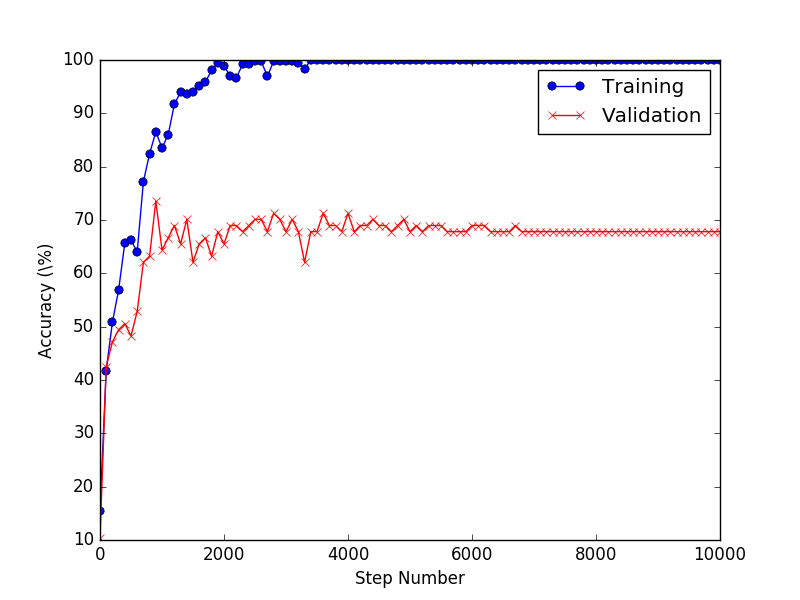
\includegraphics [trim=0 0 0 0, clip, angle=0, width=0.8\columnwidth,
	keepaspectratio]{figures/2_3_num_steps}
	\caption{Training and validation accuracy are plotted over 10,000 training steps. Validation performance levels off after 1,000 training steps, but training accuracy continues to increase. This behavior looks like overfitting, so training should be stopped early around step 1,000.} 
	\label{fig:2_3_num_steps} 
\end{figure}

The pooling layers seem to make no difference on performance.

\subsection{Part 4}
Finally, we use the network on a transformed version of the dataset.
Results in \cref{table_2_4} show that the performance is not the same for every transormation type.
For example, the original CNN only gets 10\% accuracy on inverted images, compared to 66.7\% on low contrast images (all relative to a 70.1\% accuracy on normal images).

\cref{table_2_4}'s columns show the original CNN, a CNN with Early Stopping and one with both Early Stopping and Max Pooling.
The results are not significantly different.
This aligns with the earlier observation that max pooling does not affect this problem much.
Early Stopping surprisingly didn't have much effect either.


\begin{table}[ht!]
\centering
\begin{tabular}{||c c c c||}  
 \hline
  & Regular & ES & ES \& Pooling \\
 Transformation & Val Acc (\%) & Val Acc (\%) & Val Acc (\%) \\ [0.3ex] 
 \hline\hline
 Normal & 65.5 & 70.1 & 69.0 \\ \hline
 Translated & 33.3 & 29.9 & 35.6 \\ \hline
 Brightened & 46.0 & 47.1 & 43.7 \\ \hline
 Darkened & 47.1 & 49.4 & 46.0 \\ \hline
 High Contrast & 62.1 & 63.2 & 58.6 \\ \hline
 Low Contrast & 66.7 & 66.7 & 67.8 \\ \hline
 Flipped & 42.5 & 41.4 & 44.8 \\ \hline
 Inverted & 8.0 & 10.3 & 12.6 \\ \hline
\end{tabular}
\caption{Accuracy of CNNs on transformed dataset, with Early Stopping (ES) and Max pooling.}
\label{table_2_4}
\end{table}



